\chapter{Modelowanie systemu}
\label{cha:modelowanie-systemu}

\section{Diagram przypadków użycia}
\label{sec:diagram-przypadkow-uzycia}

Diagram przypadków użycia przedstawia system z perspektywy jego użytkowników. Nie opisuje on szczegółów technicznych, struktury bazy danych ani kolejnych ekranów aplikacji, lecz pokazuje, jakie główne cele mogą realizować poszczególni aktorzy. W przypadku systemu OSK-Manager diagram obejmuje cały system na poziomie biznesowym, ponieważ dokumentowana aplikacja jest spójnym narzędziem do zarządzania ośrodkiem szkolenia kierowców.

Na diagramie wyróżniono trzy główne role użytkowników: kursanta, instruktora oraz managera OSK. Kursant korzysta z funkcji związanych z własnym kursem i lekcjami. Instruktor zarządza dostępnością oraz realizuje zajęcia przypisane do jego grafiku. Manager OSK odpowiada za część organizacyjną, czyli kursy, osoby przypisane do ośrodka, pojazdy, harmonogram oraz płatności.

\begin{figure}[H]
\centering
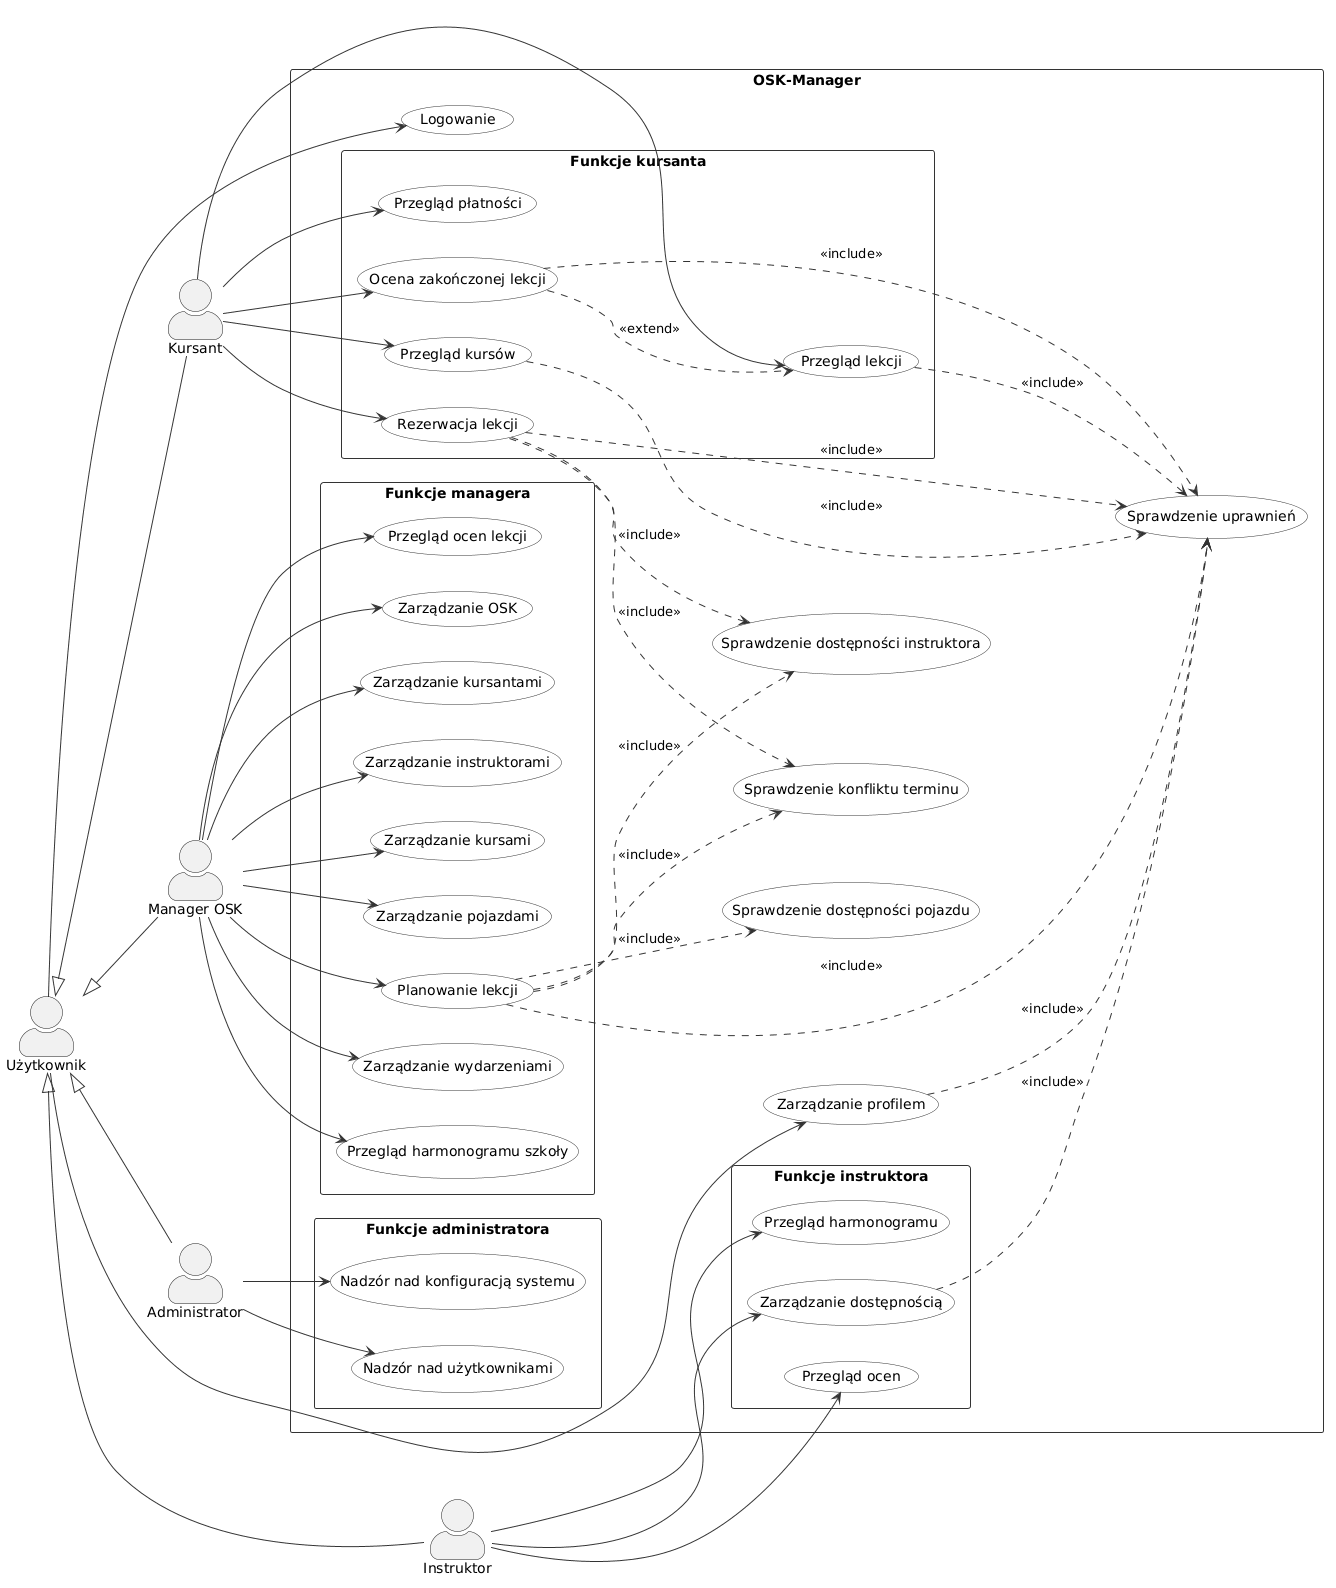
\includegraphics[width=\textwidth,height=0.72\textheight,keepaspectratio]{figures/generated/dpu.png}
\caption{Diagram przypadków użycia systemu OSK-Manager}
\label{fig:dpu-osk-manager}
\wsizsource{Opracowanie własne}
\end{figure}

Przedstawiony diagram celowo pomija szczegóły implementacyjne, takie jak konkretne endpointy API, formularze lub komponenty interfejsu. Takie elementy nie są celem diagramu przypadków użycia. W dokumentacji pełnią one rolę materiału pomocniczego dla dalszych części, przede wszystkim scenariuszy przypadków użycia oraz diagramów aktywności i sekwencji.

\section{Diagram klas}
\label{sec:diagram-klas}

Diagram klas przedstawia uproszczony model domenowy systemu OSK-Manager oraz najważniejsze relacje między obiektami. Model koncentruje się na klasach potrzebnych do opisania głównego procesu biznesowego: zarządzania szkołą jazdy, kursami, lekcjami, instruktorami, pojazdami i płatnościami. Na diagramie celowo pominięto część klas pomocniczych oraz szczegóły techniczne takie jak kontrolery, serwisy, endpointy API i komponenty interfejsu użytkownika.

\begin{figure}[H]
\centering
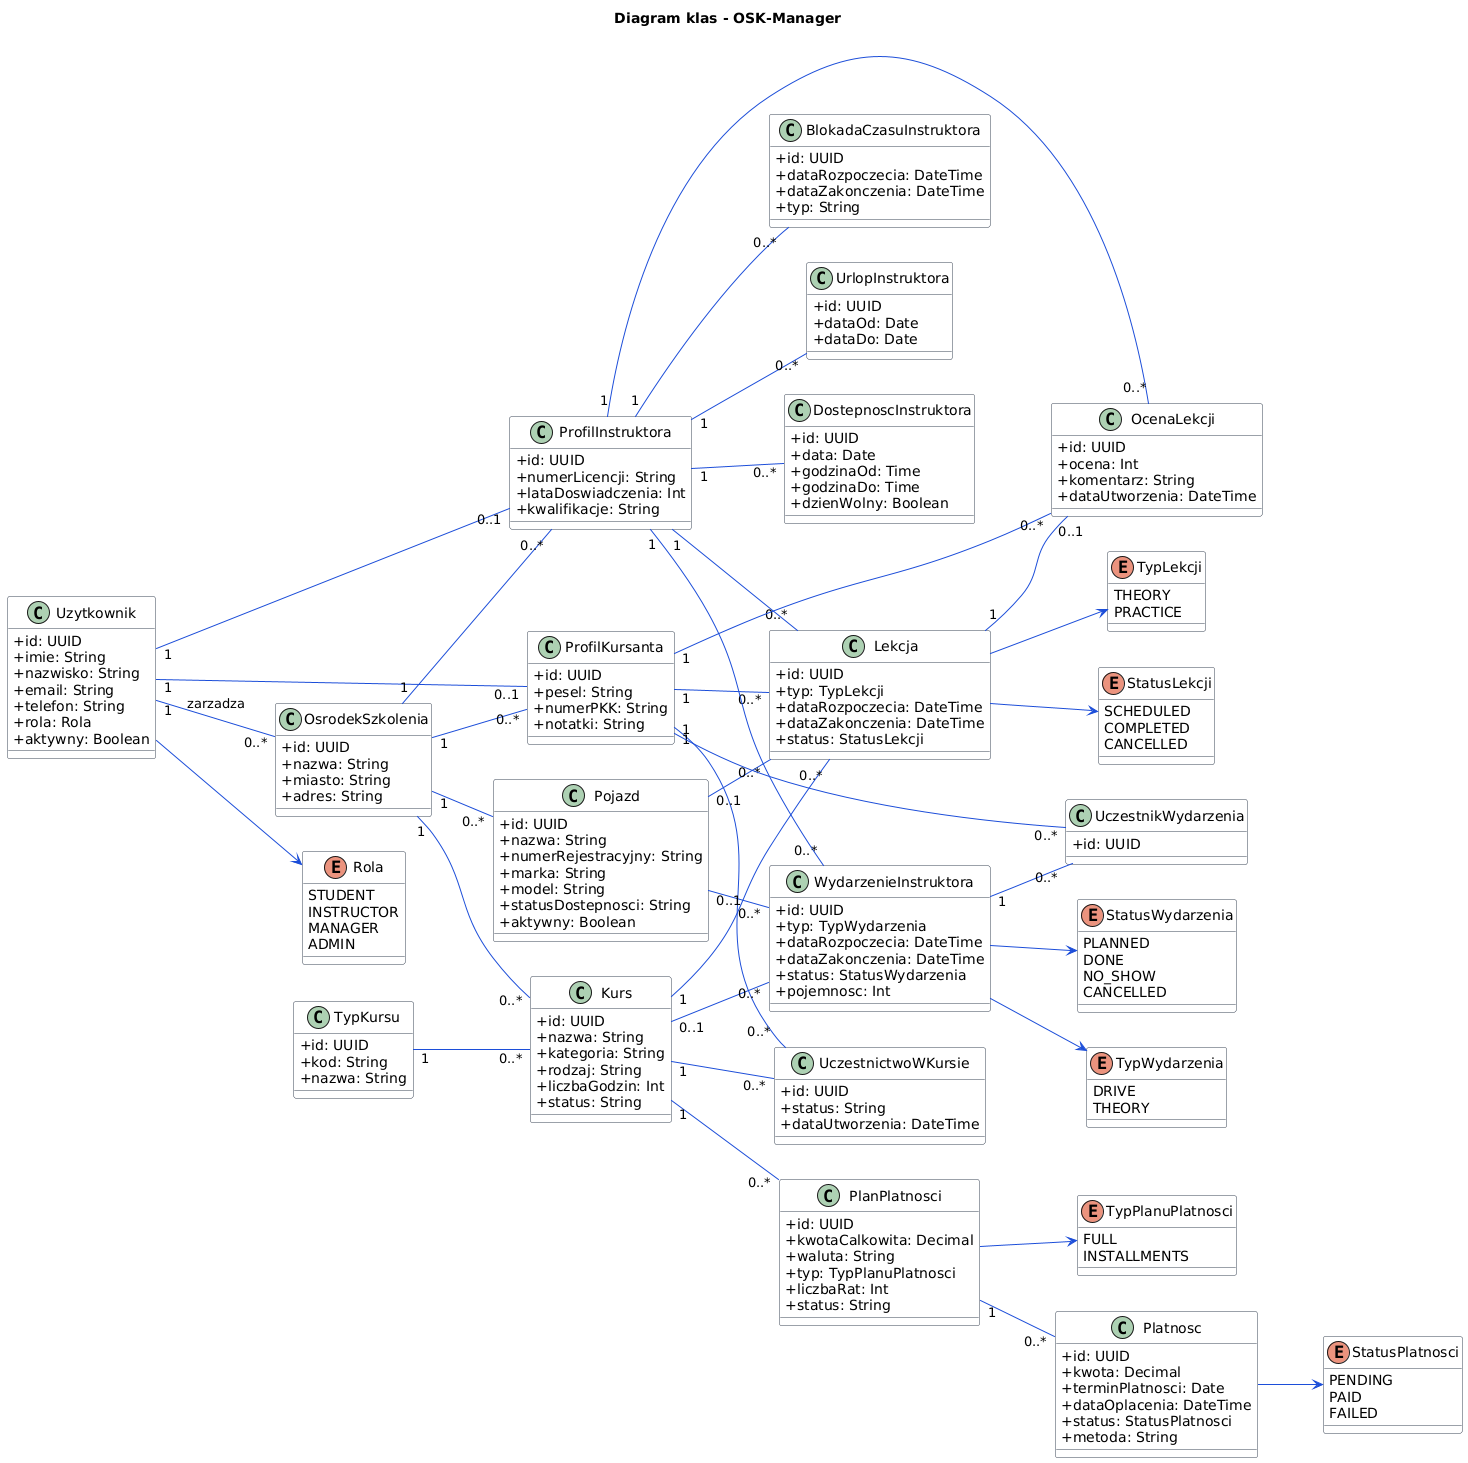
\includegraphics[width=\textwidth,height=0.76\textheight,keepaspectratio]{figures/generated/class-diagram.png}
\caption{Diagram klas systemu OSK-Manager}
\label{fig:diagram-klas-osk-manager}
\wsizsource{Opracowanie własne}
\end{figure}

Klasa \textit{Użytkownik} reprezentuje wszystkie osoby korzystające z systemu, a ich uprawnienia wynikają z przypisanej roli. Ośrodek szkolenia jest centralnym elementem modelu, ponieważ grupuje kursy, pojazdy i użytkowników. Kurs składa się z lekcji, a lekcja praktyczna może być powiązana z pojazdem. Dostępność instruktora wspiera planowanie terminów, natomiast płatności opisują podstawową część rozliczeniową kursu.

\section{Scenariusze przypadków użycia}
\label{sec:scenariusze-przypadkow-uzycia}

Poniżej przedstawiono dwa scenariusze przypadków użycia opisujące kluczowe procesy systemu OSK-Manager. Pierwszy dotyczy pracy managera OSK przy planowaniu lekcji praktycznej, natomiast drugi opisuje działanie kursanta po zakończeniu lekcji.

\subsection{Scenariusz PU-01: Zaplanowanie lekcji praktycznej}
\label{subsec:pu-planowanie-lekcji-praktycznej}

\noindent\textbf{Aktor główny:} Manager OSK.

\noindent\textbf{Cel:} Utworzenie lekcji praktycznej dla kursanta z przypisanym instruktorem, pojazdem oraz terminem.

\noindent\textbf{Warunki początkowe:}
\begin{itemize}
    \item Manager OSK jest zalogowany w systemie.
    \item W systemie istnieje aktywny kursant przypisany do wybranego kursu.
    \item W systemie istnieje instruktor oraz pojazd należący do tego samego ośrodka OSK.
    \item Instruktor ma zdefiniowaną dostępność w harmonogramie.
\end{itemize}

\noindent\textbf{Scenariusz główny:}
\begin{enumerate}
    \item Manager OSK otwiera moduł harmonogramu.
    \item System wyświetla kalendarz zajęć oraz dostępne terminy.
    \item Manager wybiera kursanta i kurs, dla którego ma zostać zaplanowana lekcja.
    \item Manager wybiera typ lekcji jako jazdę praktyczną.
    \item System prezentuje dostępnych instruktorów oraz pojazdy powiązane z danym OSK.
    \item Manager wybiera instruktora, pojazd, datę oraz godzinę rozpoczęcia lekcji.
    \item System sprawdza, czy instruktor i pojazd są dostępni w wybranym terminie.
    \item System sprawdza, czy lekcja należy do właściwego kursu oraz tego samego ośrodka OSK.
    \item Manager zatwierdza utworzenie lekcji.
    \item System zapisuje lekcję i aktualizuje harmonogram.
\end{enumerate}

\noindent\textbf{Scenariusze alternatywne:}
\begin{itemize}
    \item Jeżeli instruktor jest niedostępny, system blokuje zapis i informuje managera o konflikcie terminu.
    \item Jeżeli pojazd jest już przypisany do innej lekcji w tym samym czasie, system blokuje zapis i wymaga wyboru innego pojazdu lub terminu.
    \item Jeżeli wybrany kursant, instruktor lub pojazd nie należy do tego samego OSK, system odrzuca operację.
\end{itemize}

\noindent\textbf{Warunki końcowe:}
\begin{itemize}
    \item Lekcja praktyczna zostaje zapisana w systemie.
    \item Harmonogram kursanta i instruktora zostaje zaktualizowany.
    \item Wybrany pojazd jest oznaczony jako zajęty w czasie trwania lekcji.
\end{itemize}

\subsection{Scenariusz PU-02: Ocena zakończonej lekcji}
\label{subsec:pu-ocena-zakonczonej-lekcji}

\noindent\textbf{Aktor główny:} Kursant.

\noindent\textbf{Cel:} Wystawienie oceny zakończonej lekcji praktycznej.

\noindent\textbf{Warunki początkowe:}
\begin{itemize}
    \item Kursant jest zalogowany w systemie.
    \item Kursant ma przypisaną lekcję praktyczną.
    \item Lekcja ma status zakończony.
    \item Lekcja nie została wcześniej oceniona przez kursanta.
\end{itemize}

\noindent\textbf{Scenariusz główny:}
\begin{enumerate}
    \item Kursant otwiera widok swoich lekcji.
    \item System wyświetla listę lekcji przypisanych do kursanta.
    \item Kursant wybiera zakończoną lekcję praktyczną.
    \item System wyświetla szczegóły lekcji oraz formularz oceny.
    \item Kursant wybiera ocenę i opcjonalnie wpisuje komentarz.
    \item Kursant zatwierdza formularz.
    \item System sprawdza, czy lekcja jest zakończoną lekcją praktyczną i czy nie posiada jeszcze oceny.
    \item System zapisuje ocenę lekcji.
    \item System wyświetla potwierdzenie zapisania oceny.
\end{enumerate}

\noindent\textbf{Scenariusze alternatywne:}
\begin{itemize}
    \item Jeżeli lekcja nie jest zakończona, system nie pozwala wystawić oceny.
    \item Jeżeli lekcja jest lekcją teoretyczną, system nie udostępnia formularza oceny.
    \item Jeżeli lekcja została już oceniona, system pokazuje istniejącą ocenę i blokuje ponowne wystawienie oceny.
    \item Jeżeli kursant próbuje ocenić lekcję innego kursanta, system odmawia dostępu.
\end{itemize}

\noindent\textbf{Warunki końcowe:}
\begin{itemize}
    \item Ocena lekcji zostaje zapisana w systemie.
    \item Kursant może zobaczyć zapisaną ocenę w szczegółach lekcji.
    \item Instruktor i manager OSK mogą wykorzystać ocenę jako informację zwrotną dotyczącą jakości szkolenia.
\end{itemize}

\section{Diagramy aktywności}
\label{sec:diagramy-aktywnosci}

Diagramy aktywności przedstawiają kolejność działań wykonywanych przez użytkowników oraz system w ramach wybranych procesów biznesowych. W dokumentacji systemu OSK-Manager przygotowano dwa diagramy odpowiadające scenariuszom przypadków użycia: zaplanowaniu lekcji praktycznej oraz ocenie zakończonej lekcji.

\subsection{Diagram aktywności: zaplanowanie lekcji praktycznej}
\label{subsec:diagram-aktywnosci-planowanie-lekcji}

Pierwszy diagram przedstawia proces tworzenia lekcji praktycznej przez managera OSK. Szczególną uwagę zwrócono na kontrolę dostępności instruktora i pojazdu, ponieważ są to warunki konieczne do poprawnego zapisania zajęć w harmonogramie.

\begin{figure}[H]
\centering
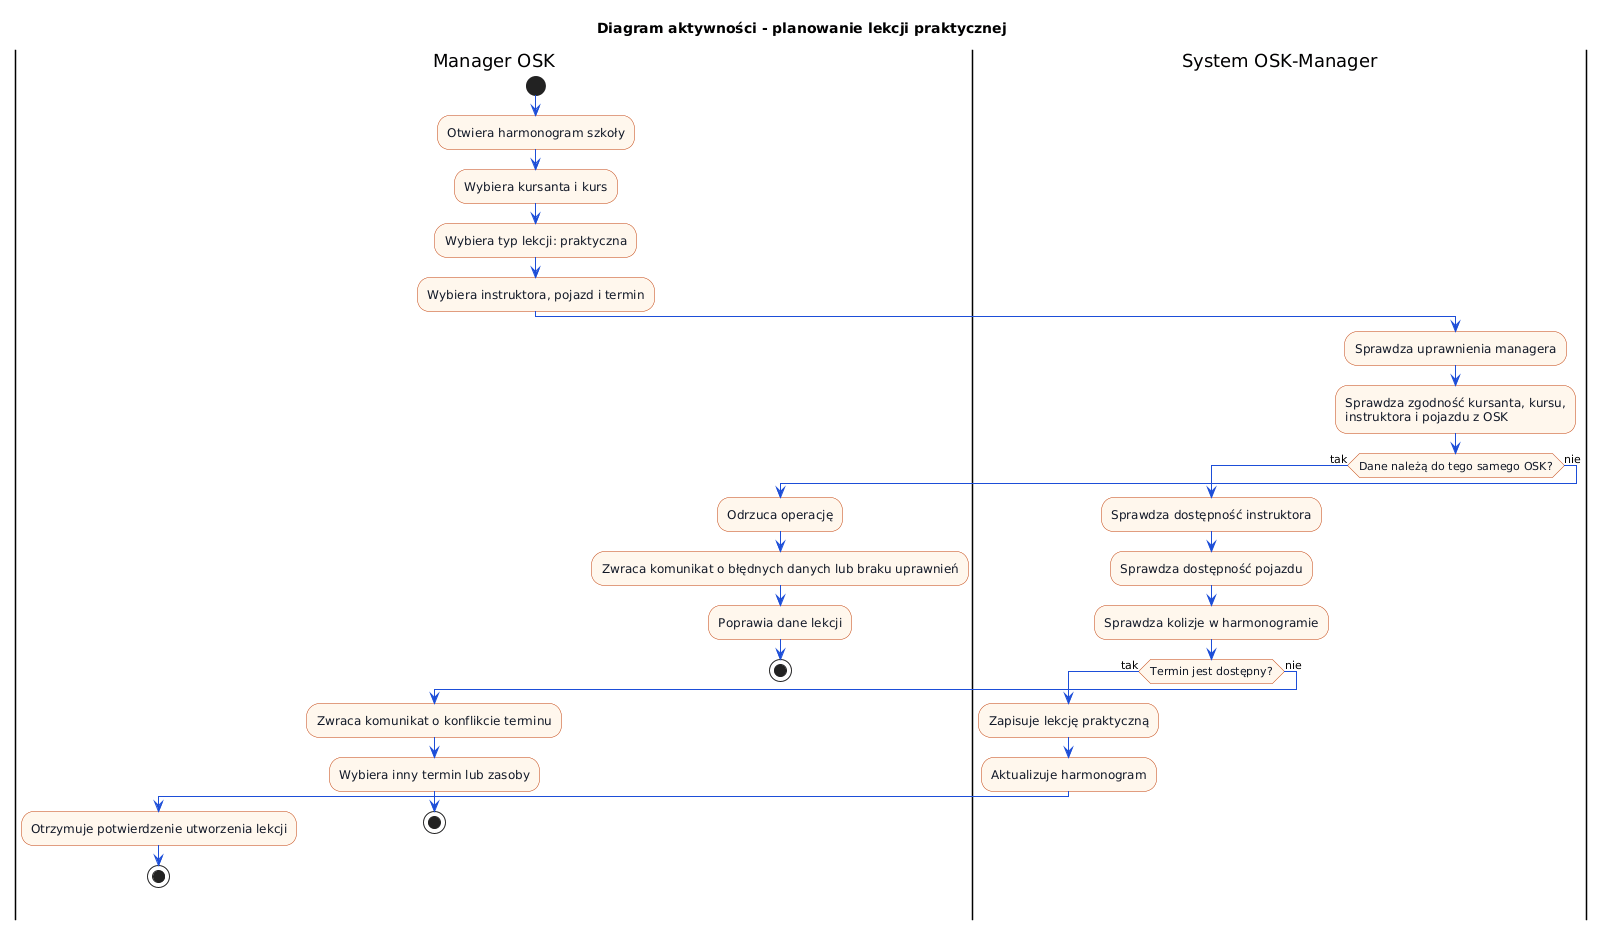
\includegraphics[width=\textwidth,height=0.76\textheight,keepaspectratio]{figures/generated/activity-plan-lesson.png}
\caption{Diagram aktywności procesu planowania lekcji praktycznej}
\label{fig:diagram-aktywnosci-planowanie-lekcji}
\wsizsource{Opracowanie własne}
\end{figure}

\subsection{Diagram aktywności: ocena zakończonej lekcji}
\label{subsec:diagram-aktywnosci-ocena-lekcji}

Drugi diagram przedstawia proces wystawienia oceny lekcji przez kursanta. Proces obejmuje sprawdzenie, czy lekcja została zakończona, czy jest lekcją praktyczną oraz czy nie została wcześniej oceniona.

\begin{figure}[H]
\centering
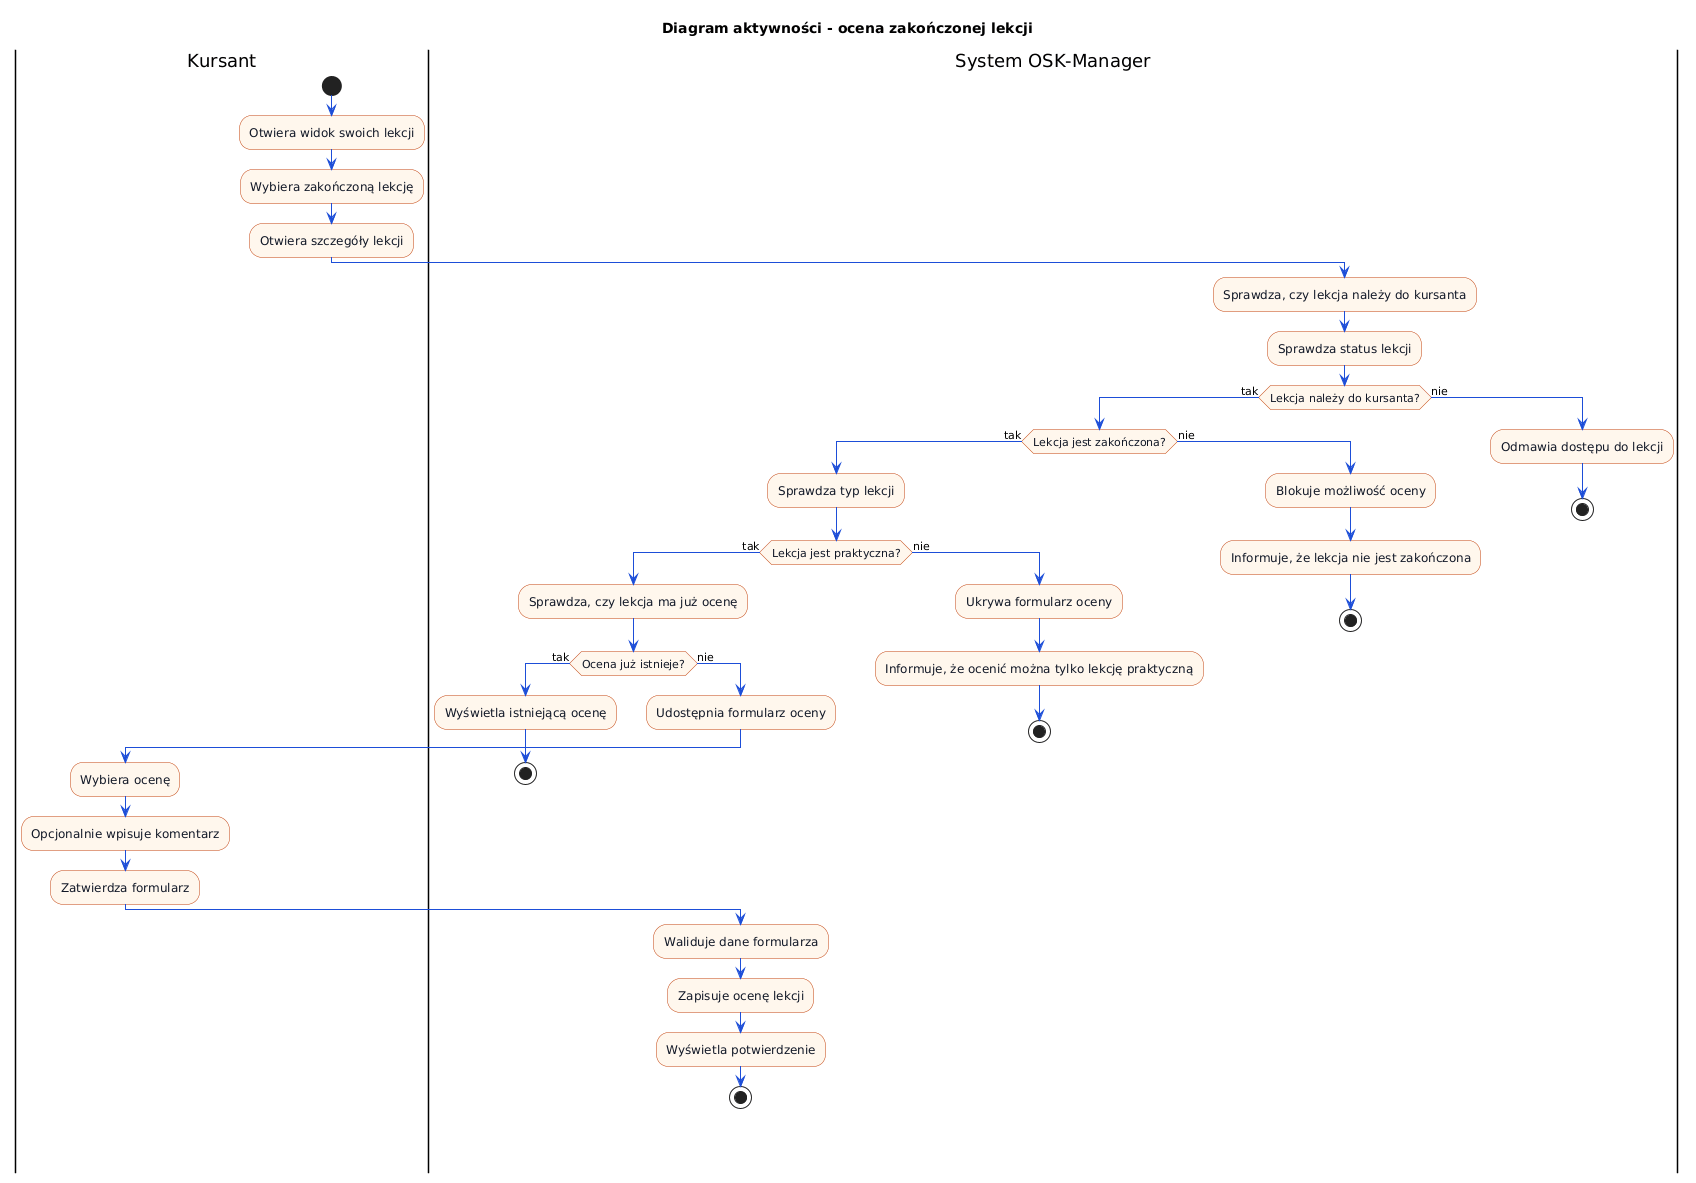
\includegraphics[width=\textwidth,height=0.76\textheight,keepaspectratio]{figures/generated/activity-rate-lesson.png}
\caption{Diagram aktywności procesu oceny zakończonej lekcji}
\label{fig:diagram-aktywnosci-ocena-lekcji}
\wsizsource{Opracowanie własne}
\end{figure}

\section{Diagramy sekwencji}
\label{sec:diagramy-sekwencji}

Diagramy sekwencji przedstawiają wymianę komunikatów pomiędzy uczestnikami procesu w kolejności czasowej. W dokumentacji systemu OSK-Manager przygotowano dwa diagramy odpowiadające kluczowym scenariuszom opisanym wcześniej: zaplanowaniu lekcji praktycznej oraz ocenie zakończonej lekcji. Diagramy pokazują uproszczoną komunikację pomiędzy użytkownikiem, interfejsem aplikacji, backendem oraz bazą danych.

\subsection{Diagram sekwencji: zaplanowanie lekcji praktycznej}
\label{subsec:diagram-sekwencji-planowanie-lekcji}

Pierwszy diagram przedstawia komunikację realizowaną podczas tworzenia lekcji praktycznej przez managera OSK. Szczególnie istotne są zapytania sprawdzające dostępność instruktora i pojazdu, ponieważ od ich wyniku zależy zapis lekcji.

\begin{figure}[H]
\centering
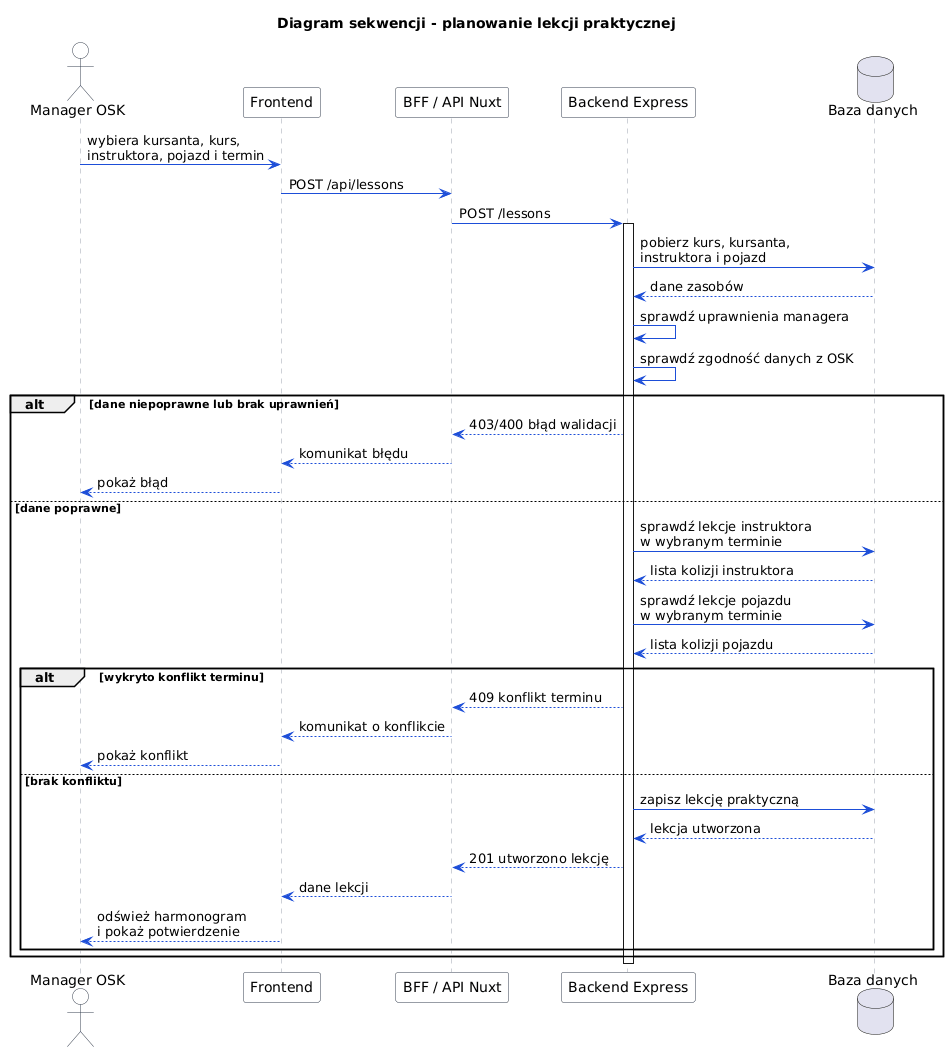
\includegraphics[width=\textwidth,height=0.76\textheight,keepaspectratio]{figures/generated/sequence-plan-lesson.png}
\caption{Diagram sekwencji procesu planowania lekcji praktycznej}
\label{fig:diagram-sekwencji-planowanie-lekcji}
\wsizsource{Opracowanie własne}
\end{figure}

\subsection{Diagram sekwencji: ocena zakończonej lekcji}
\label{subsec:diagram-sekwencji-ocena-lekcji}

Drugi diagram przedstawia komunikację podczas wystawiania oceny zakończonej lekcji przez kursanta. Backend sprawdza, czy lekcja należy do zalogowanego kursanta, czy jest zakończona, czy jest lekcją praktyczną oraz czy nie ma już zapisanej oceny.

\begin{figure}[H]
\centering
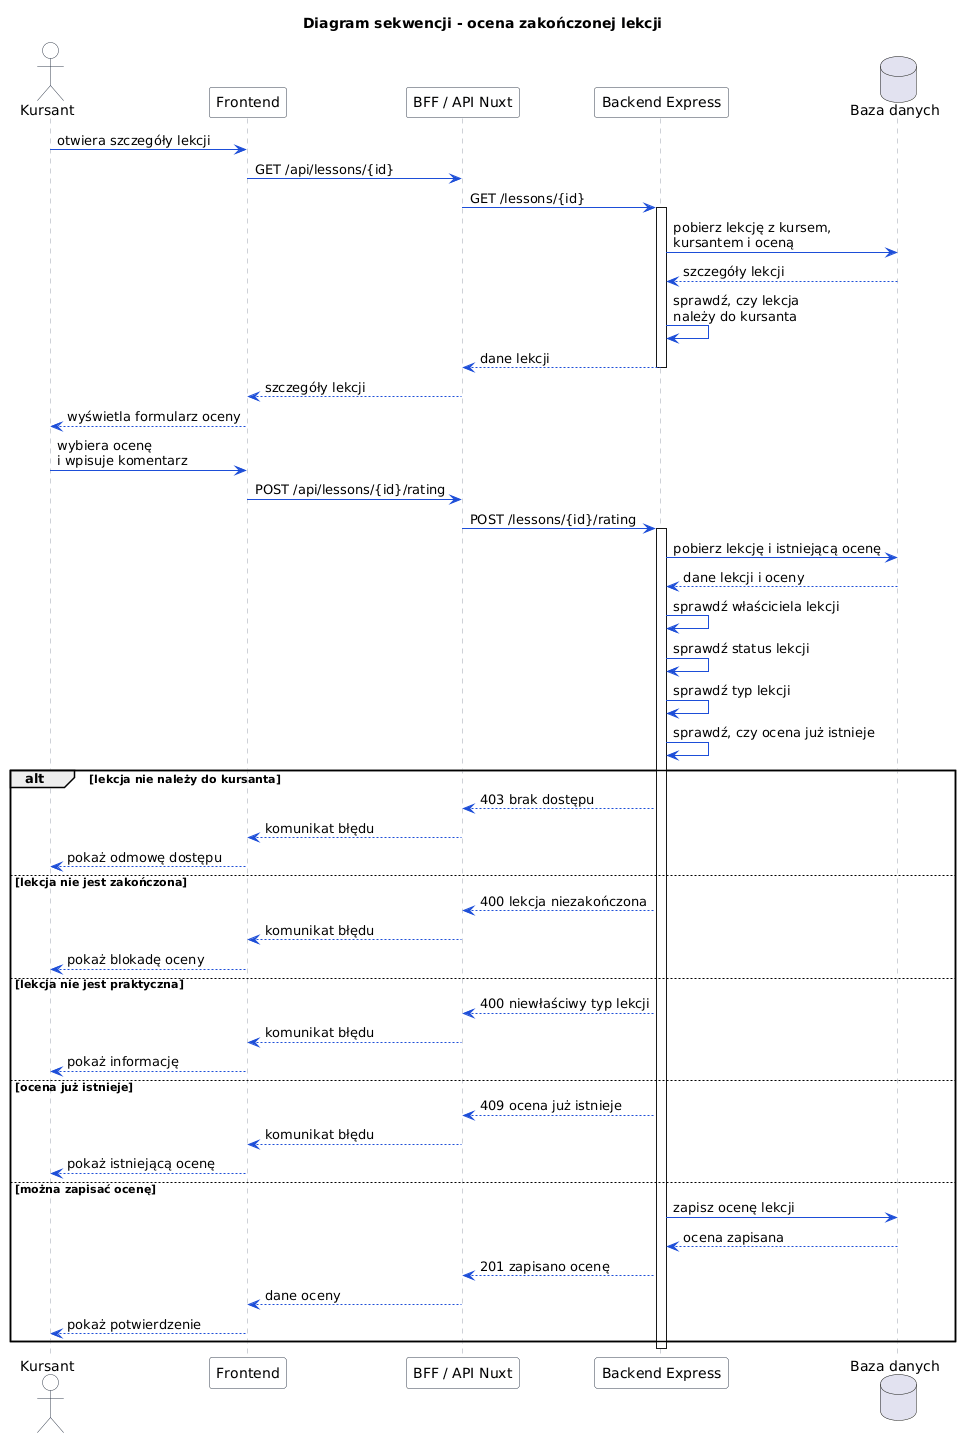
\includegraphics[width=\textwidth,height=0.76\textheight,keepaspectratio]{figures/generated/sequence-rate-lesson.png}
\caption{Diagram sekwencji procesu oceny zakończonej lekcji}
\label{fig:diagram-sekwencji-ocena-lekcji}
\wsizsource{Opracowanie własne}
\end{figure}

\section{Diagramy stanów}
\label{sec:diagramy-stanow}

Diagramy stanów pokazują możliwe stany wybranych obiektów systemu oraz zdarzenia powodujące przejścia pomiędzy nimi. W systemie OSK-Manager szczególnie istotne są cykle życia kursu oraz lekcji, ponieważ wpływają one na harmonogram, dostępność zasobów, panel kursanta oraz rozliczenia.

\subsection{Diagram stanów: kurs}
\label{subsec:diagram-stanow-kurs}

Pierwszy diagram przedstawia uproszczony cykl życia kursu. Kurs po utworzeniu jest przygotowywany organizacyjnie, następnie przechodzi w stan aktywny, a po realizacji wymaganych zajęć może zostać zakończony. W przypadku rezygnacji kursanta lub decyzji managera kurs może zostać anulowany.

\begin{figure}[H]
\centering
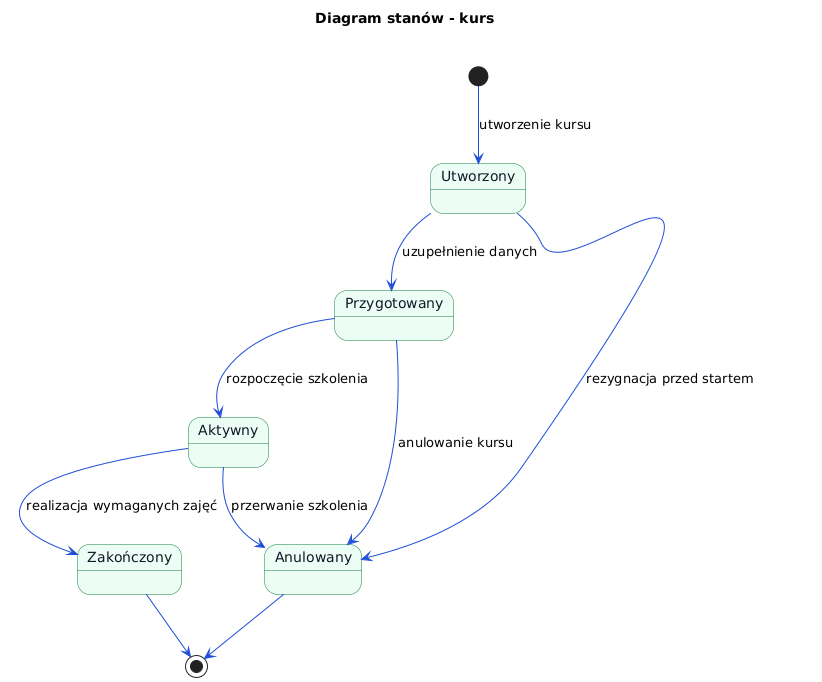
\includegraphics[width=0.78\textwidth,height=0.66\textheight,keepaspectratio]{figures/generated/state-course.png}
\caption{Diagram stanów kursu w systemie OSK-Manager}
\label{fig:diagram-stanow-kurs}
\wsizsource{Opracowanie własne}
\end{figure}

\subsection{Diagram stanów: lekcja}
\label{subsec:diagram-stanow-lekcja}

Drugi diagram przedstawia cykl życia lekcji. Lekcja po zaplanowaniu oczekuje na termin realizacji. Następnie może zostać przeprowadzona i zakończona albo anulowana przed rozpoczęciem. Dla zakończonej lekcji praktycznej możliwe jest zapisanie oceny przez kursanta.

\begin{figure}[H]
\centering
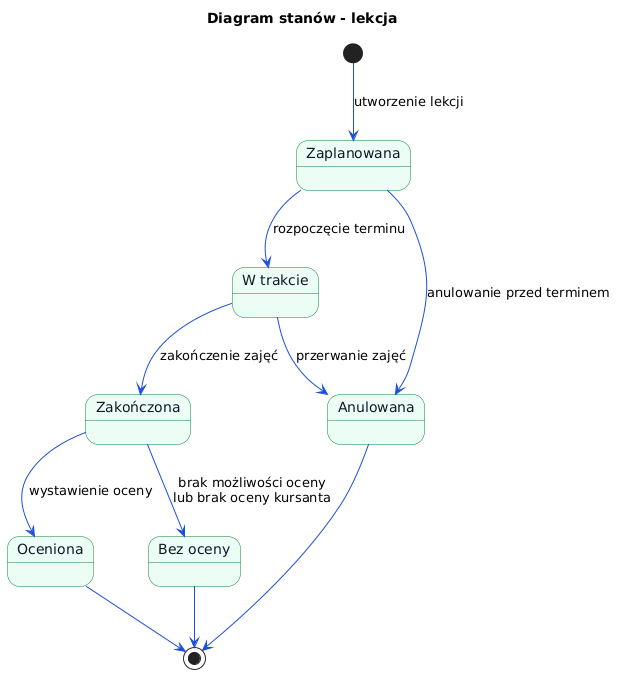
\includegraphics[width=0.78\textwidth,height=0.66\textheight,keepaspectratio]{figures/generated/state-lesson.png}
\caption{Diagram stanów lekcji w systemie OSK-Manager}
\label{fig:diagram-stanow-lekcja}
\wsizsource{Opracowanie własne}
\end{figure}
